% Generated 2020-01-10 14:19:52 -0800
\subsection{Component Types} \label{model:ComponentTypes}

\begin{figure}[ht]
  \centering
    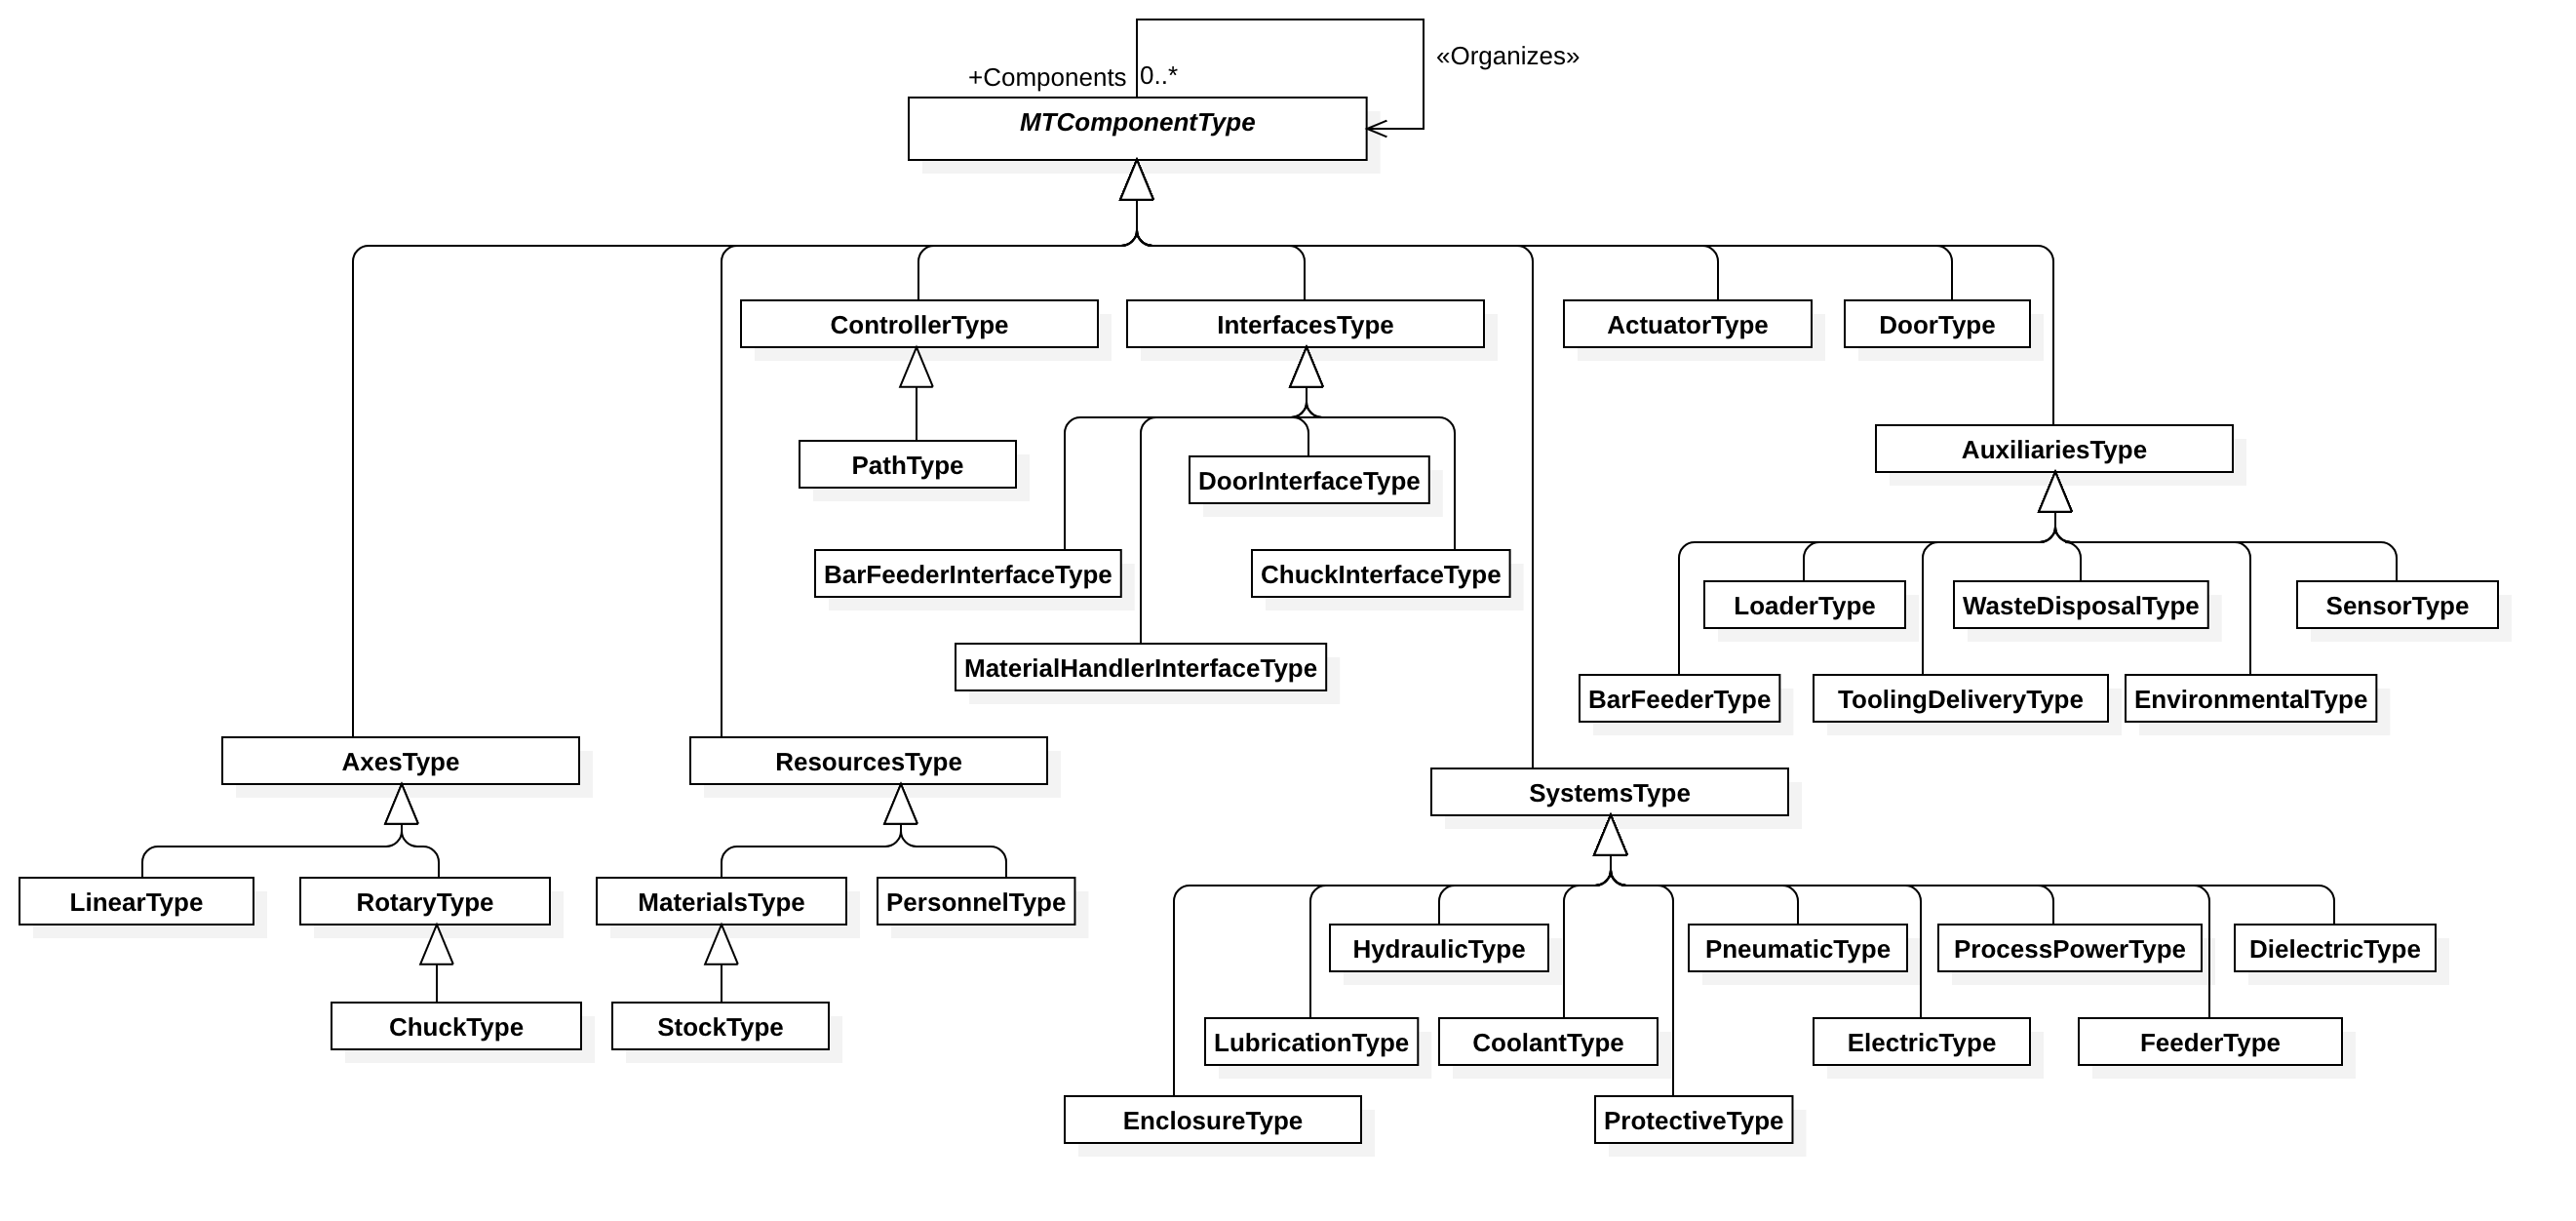
\includegraphics[width=1.0\textwidth]{./diagrams/types/ComponentTypes.png}
  \caption{Component Types Diagram}
  \label{fig:ComponentTypes}
\end{figure}

\FloatBarrier


All the sub types of components organized into top level organizational types.

\subsubsection{Defintion of \texttt{ ActuatorType}}
  \label{type:ActuatorType}

\FloatBarrier

the information for an apparatus for moving or controlling a mechanism or system

Redefined as a piece of equipment with the ability to be represented as a lower level component of a parent component element or as a composition element. See actuator type

\begin{table}[ht]
\centering 
  \caption{\texttt{ActuatorType} Definition}
  \label{table:ActuatorType}
\fontsize{9pt}{11pt}\selectfont
\tabulinesep=3pt
\begin{tabu} to 6in {|X[-1.35]|X[-0.7]|X[-1.75]|X[-1.5]|X[-1]|X[-0.7]|} \everyrow{\hline}
\hline
\rowfont\bfseries {Attribute} & \multicolumn{5}{|l|}{Value} \\
\tabucline[1.5pt]{}
BrowseName & \multicolumn{5}{|l|}{ActuatorType} \\
IsAbstract & \multicolumn{5}{|l|}{False} \\
\tabucline[1.5pt]{}
\rowfont \bfseries References & NodeClass & BrowseName & DataType & Type\-Definition & {Modeling\-Rule} \\
\multicolumn{6}{|l|}{Subtype of MTComponentType (See Components Documentation)} \\
\end{tabu}
\end{table} 


\FloatBarrier
\subsubsection{Defintion of \texttt{ AuxiliariesType}}
  \label{type:AuxiliariesType}

\FloatBarrier

representing functional sub-systems that provide supplementary or extended capabilities for a piece of equipment, 
but they are not required for the basic operation of the equipment

An XML container used to organize information for lower level elements representing functional sub-systems that provide supplementary or extended capabilities for a piece of equipment, but they are not required for the basic operation of the equipment.

\begin{table}[ht]
\centering 
  \caption{\texttt{AuxiliariesType} Definition}
  \label{table:AuxiliariesType}
\fontsize{9pt}{11pt}\selectfont
\tabulinesep=3pt
\begin{tabu} to 6in {|X[-1.35]|X[-0.7]|X[-1.75]|X[-1.5]|X[-1]|X[-0.7]|} \everyrow{\hline}
\hline
\rowfont\bfseries {Attribute} & \multicolumn{5}{|l|}{Value} \\
\tabucline[1.5pt]{}
BrowseName & \multicolumn{5}{|l|}{AuxiliariesType} \\
IsAbstract & \multicolumn{5}{|l|}{False} \\
\tabucline[1.5pt]{}
\rowfont \bfseries References & NodeClass & BrowseName & DataType & Type\-Definition & {Modeling\-Rule} \\
\multicolumn{6}{|l|}{Subtype of MTComponentType (See Components Documentation)} \\
HasSubtype & ObjectType & \multicolumn{2}{l}{BarFeederType} & \multicolumn{2}{|l|}{See section \ref{type:BarFeederType}} \\
HasSubtype & ObjectType & \multicolumn{2}{l}{EnvironmentalType} & \multicolumn{2}{|l|}{See section \ref{type:EnvironmentalType}} \\
HasSubtype & ObjectType & \multicolumn{2}{l}{LoaderType} & \multicolumn{2}{|l|}{See section \ref{type:LoaderType}} \\
HasSubtype & ObjectType & \multicolumn{2}{l}{SensorType} & \multicolumn{2}{|l|}{See section \ref{type:SensorType}} \\
HasSubtype & ObjectType & \multicolumn{2}{l}{ToolingDeliveryType} & \multicolumn{2}{|l|}{See section \ref{type:ToolingDeliveryType}} \\
HasSubtype & ObjectType & \multicolumn{2}{l}{WasteDisposalType} & \multicolumn{2}{|l|}{See section \ref{type:WasteDisposalType}} \\
\end{tabu}
\end{table} 


\FloatBarrier
\subsubsection{Defintion of \texttt{ BarFeederType}}
  \label{type:BarFeederType}

\FloatBarrier

a unit involved in delivering bar stock to a piece of equipment.

barfeeder is an XML container that represents the information for a unit involved in delivering bar stock to a piece of equipment.

\begin{table}[ht]
\centering 
  \caption{\texttt{BarFeederType} Definition}
  \label{table:BarFeederType}
\fontsize{9pt}{11pt}\selectfont
\tabulinesep=3pt
\begin{tabu} to 6in {|X[-1.35]|X[-0.7]|X[-1.75]|X[-1.5]|X[-1]|X[-0.7]|} \everyrow{\hline}
\hline
\rowfont\bfseries {Attribute} & \multicolumn{5}{|l|}{Value} \\
\tabucline[1.5pt]{}
BrowseName & \multicolumn{5}{|l|}{BarFeederType} \\
IsAbstract & \multicolumn{5}{|l|}{False} \\
\tabucline[1.5pt]{}
\rowfont \bfseries References & NodeClass & BrowseName & DataType & Type\-Definition & {Modeling\-Rule} \\
\multicolumn{6}{|l|}{Subtype of AuxiliariesType (See section \ref{type:AuxiliariesType})} \\
\end{tabu}
\end{table} 


\FloatBarrier
\subsubsection{Defintion of \texttt{ EnvironmentalType}}
  \label{type:EnvironmentalType}

\FloatBarrier

the information for a unit or function involved in monitoring, managing, or conditioning 
the environment around or within a piece of equipment.

environmental is an XML container that represents the information for a unit or function involved in monitoring, managing, or conditioning the environment around or within a piece of equipment.

\begin{table}[ht]
\centering 
  \caption{\texttt{EnvironmentalType} Definition}
  \label{table:EnvironmentalType}
\fontsize{9pt}{11pt}\selectfont
\tabulinesep=3pt
\begin{tabu} to 6in {|X[-1.35]|X[-0.7]|X[-1.75]|X[-1.5]|X[-1]|X[-0.7]|} \everyrow{\hline}
\hline
\rowfont\bfseries {Attribute} & \multicolumn{5}{|l|}{Value} \\
\tabucline[1.5pt]{}
BrowseName & \multicolumn{5}{|l|}{EnvironmentalType} \\
IsAbstract & \multicolumn{5}{|l|}{False} \\
\tabucline[1.5pt]{}
\rowfont \bfseries References & NodeClass & BrowseName & DataType & Type\-Definition & {Modeling\-Rule} \\
\multicolumn{6}{|l|}{Subtype of AuxiliariesType (See section \ref{type:AuxiliariesType})} \\
\end{tabu}
\end{table} 


\FloatBarrier
\subsubsection{Defintion of \texttt{ LoaderType}}
  \label{type:LoaderType}

\FloatBarrier

the information for a unit comprised of all the parts involved in moving and distributing materials, 
parts, tooling, and other items to or from a piece of equipment

loader is an XML container that represents the information for a unit comprised of all the parts involved in moving and distributing materials, parts, tooling, and other items to or from a piece of equipment.

\begin{table}[ht]
\centering 
  \caption{\texttt{LoaderType} Definition}
  \label{table:LoaderType}
\fontsize{9pt}{11pt}\selectfont
\tabulinesep=3pt
\begin{tabu} to 6in {|X[-1.35]|X[-0.7]|X[-1.75]|X[-1.5]|X[-1]|X[-0.7]|} \everyrow{\hline}
\hline
\rowfont\bfseries {Attribute} & \multicolumn{5}{|l|}{Value} \\
\tabucline[1.5pt]{}
BrowseName & \multicolumn{5}{|l|}{LoaderType} \\
IsAbstract & \multicolumn{5}{|l|}{False} \\
\tabucline[1.5pt]{}
\rowfont \bfseries References & NodeClass & BrowseName & DataType & Type\-Definition & {Modeling\-Rule} \\
\multicolumn{6}{|l|}{Subtype of AuxiliariesType (See section \ref{type:AuxiliariesType})} \\
\end{tabu}
\end{table} 


\FloatBarrier
\subsubsection{Defintion of \texttt{ SensorType}}
  \label{type:SensorType}

\FloatBarrier

the information for a piece of equipment that responds to a physical stimulus and transmits a resulting impulse or value from a sensing unit

The sensor unit is modeled as a lower level component called sensor.

\begin{table}[ht]
\centering 
  \caption{\texttt{SensorType} Definition}
  \label{table:SensorType}
\fontsize{9pt}{11pt}\selectfont
\tabulinesep=3pt
\begin{tabu} to 6in {|X[-1.35]|X[-0.7]|X[-1.75]|X[-1.5]|X[-1]|X[-0.7]|} \everyrow{\hline}
\hline
\rowfont\bfseries {Attribute} & \multicolumn{5}{|l|}{Value} \\
\tabucline[1.5pt]{}
BrowseName & \multicolumn{5}{|l|}{SensorType} \\
IsAbstract & \multicolumn{5}{|l|}{False} \\
\tabucline[1.5pt]{}
\rowfont \bfseries References & NodeClass & BrowseName & DataType & Type\-Definition & {Modeling\-Rule} \\
\multicolumn{6}{|l|}{Subtype of AuxiliariesType (See section \ref{type:AuxiliariesType})} \\
\end{tabu}
\end{table} 


\FloatBarrier
\subsubsection{Defintion of \texttt{ ToolingDeliveryType}}
  \label{type:ToolingDeliveryType}

\FloatBarrier

a unit involved in managing, positioning, storing, and delivering tooling within a piece of equipment.

toolingdelivery is an XML container that represents the information for a unit involved in managing, positioning, storing, and delivering tooling within a piece of equipment.


\begin{table}[ht]
\centering 
  \caption{\texttt{ToolingDeliveryType} Definition}
  \label{table:ToolingDeliveryType}
\fontsize{9pt}{11pt}\selectfont
\tabulinesep=3pt
\begin{tabu} to 6in {|X[-1.35]|X[-0.7]|X[-1.75]|X[-1.5]|X[-1]|X[-0.7]|} \everyrow{\hline}
\hline
\rowfont\bfseries {Attribute} & \multicolumn{5}{|l|}{Value} \\
\tabucline[1.5pt]{}
BrowseName & \multicolumn{5}{|l|}{ToolingDeliveryType} \\
IsAbstract & \multicolumn{5}{|l|}{False} \\
\tabucline[1.5pt]{}
\rowfont \bfseries References & NodeClass & BrowseName & DataType & Type\-Definition & {Modeling\-Rule} \\
\multicolumn{6}{|l|}{Subtype of AuxiliariesType (See section \ref{type:AuxiliariesType})} \\
\end{tabu}
\end{table} 


\FloatBarrier
\subsubsection{Defintion of \texttt{ WasteDisposalType}}
  \label{type:WasteDisposalType}

\FloatBarrier

the information for a unit comprised of all the parts involved in removing manufacturing byproducts from a piece of equipment

wastedisposal is an XML container that represents the information for a unit comprised of all the parts involved in removing manufacturing byproducts from a piece of equipment.


\begin{table}[ht]
\centering 
  \caption{\texttt{WasteDisposalType} Definition}
  \label{table:WasteDisposalType}
\fontsize{9pt}{11pt}\selectfont
\tabulinesep=3pt
\begin{tabu} to 6in {|X[-1.35]|X[-0.7]|X[-1.75]|X[-1.5]|X[-1]|X[-0.7]|} \everyrow{\hline}
\hline
\rowfont\bfseries {Attribute} & \multicolumn{5}{|l|}{Value} \\
\tabucline[1.5pt]{}
BrowseName & \multicolumn{5}{|l|}{WasteDisposalType} \\
IsAbstract & \multicolumn{5}{|l|}{False} \\
\tabucline[1.5pt]{}
\rowfont \bfseries References & NodeClass & BrowseName & DataType & Type\-Definition & {Modeling\-Rule} \\
\multicolumn{6}{|l|}{Subtype of AuxiliariesType (See section \ref{type:AuxiliariesType})} \\
\end{tabu}
\end{table} 


\FloatBarrier
\subsubsection{Defintion of \texttt{ AxesType}}
  \label{type:AxesType}

\FloatBarrier

Organizes parts of the device that perform linear or rotational motion

An XML container used to organize the structural element of a piece of equipment that perform linear or rotational motion.

\begin{table}[ht]
\centering 
  \caption{\texttt{AxesType} Definition}
  \label{table:AxesType}
\fontsize{9pt}{11pt}\selectfont
\tabulinesep=3pt
\begin{tabu} to 6in {|X[-1.35]|X[-0.7]|X[-1.75]|X[-1.5]|X[-1]|X[-0.7]|} \everyrow{\hline}
\hline
\rowfont\bfseries {Attribute} & \multicolumn{5}{|l|}{Value} \\
\tabucline[1.5pt]{}
BrowseName & \multicolumn{5}{|l|}{AxesType} \\
IsAbstract & \multicolumn{5}{|l|}{False} \\
\tabucline[1.5pt]{}
\rowfont \bfseries References & NodeClass & BrowseName & DataType & Type\-Definition & {Modeling\-Rule} \\
\multicolumn{6}{|l|}{Subtype of MTComponentType (See Components Documentation)} \\
HasSubtype & ObjectType & \multicolumn{2}{l}{LinearType} & \multicolumn{2}{|l|}{See section \ref{type:LinearType}} \\
HasSubtype & ObjectType & \multicolumn{2}{l}{RotaryType} & \multicolumn{2}{|l|}{See section \ref{type:RotaryType}} \\
\end{tabu}
\end{table} 


\FloatBarrier
\subsubsection{Defintion of \texttt{ LinearType}}
  \label{type:LinearType}

\FloatBarrier

the movement of a physical piece of equipment, or a portion of the equipment, in a straight line.

A linear axis represents the movement of a physical piece of equipment, or a portion of the equipment, in a straight line. 

\begin{table}[ht]
\centering 
  \caption{\texttt{LinearType} Definition}
  \label{table:LinearType}
\fontsize{9pt}{11pt}\selectfont
\tabulinesep=3pt
\begin{tabu} to 6in {|X[-1.35]|X[-0.7]|X[-1.75]|X[-1.5]|X[-1]|X[-0.7]|} \everyrow{\hline}
\hline
\rowfont\bfseries {Attribute} & \multicolumn{5}{|l|}{Value} \\
\tabucline[1.5pt]{}
BrowseName & \multicolumn{5}{|l|}{LinearType} \\
IsAbstract & \multicolumn{5}{|l|}{False} \\
\tabucline[1.5pt]{}
\rowfont \bfseries References & NodeClass & BrowseName & DataType & Type\-Definition & {Modeling\-Rule} \\
\multicolumn{6}{|l|}{Subtype of AxesType (See section \ref{type:AxesType})} \\
\end{tabu}
\end{table} 


\FloatBarrier
\subsubsection{Defintion of \texttt{ RotaryType}}
  \label{type:RotaryType}

\FloatBarrier

rotary movement of a physical piece of equipment or a portion of the equipment.

A rotary axis represents any non-linear or rotary movement of a physical piece of equipment or a portion of the equipment. 

\begin{table}[ht]
\centering 
  \caption{\texttt{RotaryType} Definition}
  \label{table:RotaryType}
\fontsize{9pt}{11pt}\selectfont
\tabulinesep=3pt
\begin{tabu} to 6in {|X[-1.35]|X[-0.7]|X[-1.75]|X[-1.5]|X[-1]|X[-0.7]|} \everyrow{\hline}
\hline
\rowfont\bfseries {Attribute} & \multicolumn{5}{|l|}{Value} \\
\tabucline[1.5pt]{}
BrowseName & \multicolumn{5}{|l|}{RotaryType} \\
IsAbstract & \multicolumn{5}{|l|}{False} \\
\tabucline[1.5pt]{}
\rowfont \bfseries References & NodeClass & BrowseName & DataType & Type\-Definition & {Modeling\-Rule} \\
\multicolumn{6}{|l|}{Subtype of AxesType (See section \ref{type:AxesType})} \\
HasSubtype & ObjectType & \multicolumn{2}{l}{ChuckType} & \multicolumn{2}{|l|}{See section \ref{type:ChuckType}} \\
\end{tabu}
\end{table} 


\FloatBarrier
\subsubsection{Defintion of \texttt{ ChuckType}}
  \label{type:ChuckType}

\FloatBarrier

provides the information about a mechanism that holds a part or stock material in place

Chuck is an XML container that provides the information about a mechanism that holds a part or stock material in place.

\begin{table}[ht]
\centering 
  \caption{\texttt{ChuckType} Definition}
  \label{table:ChuckType}
\fontsize{9pt}{11pt}\selectfont
\tabulinesep=3pt
\begin{tabu} to 6in {|X[-1.35]|X[-0.7]|X[-1.75]|X[-1.5]|X[-1]|X[-0.7]|} \everyrow{\hline}
\hline
\rowfont\bfseries {Attribute} & \multicolumn{5}{|l|}{Value} \\
\tabucline[1.5pt]{}
BrowseName & \multicolumn{5}{|l|}{ChuckType} \\
IsAbstract & \multicolumn{5}{|l|}{False} \\
\tabucline[1.5pt]{}
\rowfont \bfseries References & NodeClass & BrowseName & DataType & Type\-Definition & {Modeling\-Rule} \\
\multicolumn{6}{|l|}{Subtype of RotaryType (See section \ref{type:RotaryType})} \\
\end{tabu}
\end{table} 


\FloatBarrier
\subsubsection{Defintion of \texttt{ ControllerType}}
  \label{type:ControllerType}

\FloatBarrier

intelligent or computational function within a piece of equipment

An XML container used to organize information about an intelligent or computational function within a piece of equipment.

\begin{table}[ht]
\centering 
  \caption{\texttt{ControllerType} Definition}
  \label{table:ControllerType}
\fontsize{9pt}{11pt}\selectfont
\tabulinesep=3pt
\begin{tabu} to 6in {|X[-1.35]|X[-0.7]|X[-1.75]|X[-1.5]|X[-1]|X[-0.7]|} \everyrow{\hline}
\hline
\rowfont\bfseries {Attribute} & \multicolumn{5}{|l|}{Value} \\
\tabucline[1.5pt]{}
BrowseName & \multicolumn{5}{|l|}{ControllerType} \\
IsAbstract & \multicolumn{5}{|l|}{False} \\
\tabucline[1.5pt]{}
\rowfont \bfseries References & NodeClass & BrowseName & DataType & Type\-Definition & {Modeling\-Rule} \\
\multicolumn{6}{|l|}{Subtype of MTComponentType (See Components Documentation)} \\
HasSubtype & ObjectType & \multicolumn{2}{l}{PathType} & \multicolumn{2}{|l|}{See section \ref{type:PathType}} \\
\end{tabu}
\end{table} 


\FloatBarrier
\subsubsection{Defintion of \texttt{ PathType}}
  \label{type:PathType}

\FloatBarrier

information for an independent operation or function within a \mtuatype{ControllerType}

path is an XML container that represents the information for an independent operation or function within a controller.

\begin{table}[ht]
\centering 
  \caption{\texttt{PathType} Definition}
  \label{table:PathType}
\fontsize{9pt}{11pt}\selectfont
\tabulinesep=3pt
\begin{tabu} to 6in {|X[-1.35]|X[-0.7]|X[-1.75]|X[-1.5]|X[-1]|X[-0.7]|} \everyrow{\hline}
\hline
\rowfont\bfseries {Attribute} & \multicolumn{5}{|l|}{Value} \\
\tabucline[1.5pt]{}
BrowseName & \multicolumn{5}{|l|}{PathType} \\
IsAbstract & \multicolumn{5}{|l|}{False} \\
\tabucline[1.5pt]{}
\rowfont \bfseries References & NodeClass & BrowseName & DataType & Type\-Definition & {Modeling\-Rule} \\
\multicolumn{6}{|l|}{Subtype of ControllerType (See section \ref{type:ControllerType})} \\
\end{tabu}
\end{table} 


\FloatBarrier
\subsubsection{Defintion of \texttt{ DoorType}}
  \label{type:DoorType}

\FloatBarrier

the information for a mechanical mechanism or closure that can cover, for example, a physical access portal into a piece of equipment

door component is an XML container that represents the information for a mechanical mechanism or closure that can cover.

\begin{table}[ht]
\centering 
  \caption{\texttt{DoorType} Definition}
  \label{table:DoorType}
\fontsize{9pt}{11pt}\selectfont
\tabulinesep=3pt
\begin{tabu} to 6in {|X[-1.35]|X[-0.7]|X[-1.75]|X[-1.5]|X[-1]|X[-0.7]|} \everyrow{\hline}
\hline
\rowfont\bfseries {Attribute} & \multicolumn{5}{|l|}{Value} \\
\tabucline[1.5pt]{}
BrowseName & \multicolumn{5}{|l|}{DoorType} \\
IsAbstract & \multicolumn{5}{|l|}{False} \\
\tabucline[1.5pt]{}
\rowfont \bfseries References & NodeClass & BrowseName & DataType & Type\-Definition & {Modeling\-Rule} \\
\multicolumn{6}{|l|}{Subtype of MTComponentType (See Components Documentation)} \\
\end{tabu}
\end{table} 


\FloatBarrier
\subsubsection{Defintion of \texttt{ InterfacesType}}
  \label{type:InterfacesType}

\FloatBarrier



An XML container that organizes information used to coordinate actions and activities between pieces of equipment that communicate information between each other. 

\begin{table}[ht]
\centering 
  \caption{\texttt{InterfacesType} Definition}
  \label{table:InterfacesType}
\fontsize{9pt}{11pt}\selectfont
\tabulinesep=3pt
\begin{tabu} to 6in {|X[-1.35]|X[-0.7]|X[-1.75]|X[-1.5]|X[-1]|X[-0.7]|} \everyrow{\hline}
\hline
\rowfont\bfseries {Attribute} & \multicolumn{5}{|l|}{Value} \\
\tabucline[1.5pt]{}
BrowseName & \multicolumn{5}{|l|}{InterfacesType} \\
IsAbstract & \multicolumn{5}{|l|}{False} \\
\tabucline[1.5pt]{}
\rowfont \bfseries References & NodeClass & BrowseName & DataType & Type\-Definition & {Modeling\-Rule} \\
\multicolumn{6}{|l|}{Subtype of MTComponentType (See Components Documentation)} \\
HasSubtype & ObjectType & \multicolumn{2}{l}{BarFeederInterfaceType} & \multicolumn{2}{|l|}{See section \ref{type:BarFeederInterfaceType}} \\
HasSubtype & ObjectType & \multicolumn{2}{l}{ChuckInterfaceType} & \multicolumn{2}{|l|}{See section \ref{type:ChuckInterfaceType}} \\
HasSubtype & ObjectType & \multicolumn{2}{l}{DoorInterfaceType} & \multicolumn{2}{|l|}{See section \ref{type:DoorInterfaceType}} \\
HasSubtype & ObjectType & \multicolumn{2}{l}{MaterialHandlerInterfaceType} & \multicolumn{2}{|l|}{See section \ref{type:MaterialHandlerInterfaceType}} \\
\end{tabu}
\end{table} 


\FloatBarrier
\subsubsection{Defintion of \texttt{ BarFeederInterfaceType}}
  \label{type:BarFeederInterfaceType}

\FloatBarrier

information used to coordinate the operations between a Bar Feeder and another piece of equipment

barfeederinterface provides the set of information used to coordinate the operations between a Bar Feeder and another piece of equipment.  

\begin{table}[ht]
\centering 
  \caption{\texttt{BarFeederInterfaceType} Definition}
  \label{table:BarFeederInterfaceType}
\fontsize{9pt}{11pt}\selectfont
\tabulinesep=3pt
\begin{tabu} to 6in {|X[-1.35]|X[-0.7]|X[-1.75]|X[-1.5]|X[-1]|X[-0.7]|} \everyrow{\hline}
\hline
\rowfont\bfseries {Attribute} & \multicolumn{5}{|l|}{Value} \\
\tabucline[1.5pt]{}
BrowseName & \multicolumn{5}{|l|}{BarFeederInterfaceType} \\
IsAbstract & \multicolumn{5}{|l|}{False} \\
\tabucline[1.5pt]{}
\rowfont \bfseries References & NodeClass & BrowseName & DataType & Type\-Definition & {Modeling\-Rule} \\
\multicolumn{6}{|l|}{Subtype of InterfacesType (See section \ref{type:InterfacesType})} \\
\end{tabu}
\end{table} 


\FloatBarrier
\subsubsection{Defintion of \texttt{ ChuckInterfaceType}}
  \label{type:ChuckInterfaceType}

\FloatBarrier

information used to coordinate the operations between two pieces of equipment, one of which controls the operation of a chuck

chuckinterface provides the set of information used to coordinate the operations between two pieces of equipment, one of which controls the operation of a chuck.  

\begin{table}[ht]
\centering 
  \caption{\texttt{ChuckInterfaceType} Definition}
  \label{table:ChuckInterfaceType}
\fontsize{9pt}{11pt}\selectfont
\tabulinesep=3pt
\begin{tabu} to 6in {|X[-1.35]|X[-0.7]|X[-1.75]|X[-1.5]|X[-1]|X[-0.7]|} \everyrow{\hline}
\hline
\rowfont\bfseries {Attribute} & \multicolumn{5}{|l|}{Value} \\
\tabucline[1.5pt]{}
BrowseName & \multicolumn{5}{|l|}{ChuckInterfaceType} \\
IsAbstract & \multicolumn{5}{|l|}{False} \\
\tabucline[1.5pt]{}
\rowfont \bfseries References & NodeClass & BrowseName & DataType & Type\-Definition & {Modeling\-Rule} \\
\multicolumn{6}{|l|}{Subtype of InterfacesType (See section \ref{type:InterfacesType})} \\
\end{tabu}
\end{table} 


\FloatBarrier
\subsubsection{Defintion of \texttt{ DoorInterfaceType}}
  \label{type:DoorInterfaceType}

\FloatBarrier

information used to coordinate the operations between two pieces of equipment, one of which controls the operation of a door

doorinterface provides the set of information used to coordinate the operations between two pieces of equipment, one of which controls the operation of a door. 

\begin{table}[ht]
\centering 
  \caption{\texttt{DoorInterfaceType} Definition}
  \label{table:DoorInterfaceType}
\fontsize{9pt}{11pt}\selectfont
\tabulinesep=3pt
\begin{tabu} to 6in {|X[-1.35]|X[-0.7]|X[-1.75]|X[-1.5]|X[-1]|X[-0.7]|} \everyrow{\hline}
\hline
\rowfont\bfseries {Attribute} & \multicolumn{5}{|l|}{Value} \\
\tabucline[1.5pt]{}
BrowseName & \multicolumn{5}{|l|}{DoorInterfaceType} \\
IsAbstract & \multicolumn{5}{|l|}{False} \\
\tabucline[1.5pt]{}
\rowfont \bfseries References & NodeClass & BrowseName & DataType & Type\-Definition & {Modeling\-Rule} \\
\multicolumn{6}{|l|}{Subtype of InterfacesType (See section \ref{type:InterfacesType})} \\
\end{tabu}
\end{table} 


\FloatBarrier
\subsubsection{Defintion of \texttt{ MaterialHandlerInterfaceType}}
  \label{type:MaterialHandlerInterfaceType}

\FloatBarrier

set of information used to coordinate the operations between a piece of equipment
and another associated piece of equipment used to automatically handle various types of 
materials or services associated with the original piece of equipment

materialhandlerinterface provides the set of information used to coordinate the operations between a piece of equipment and another associated piece of equipment used to automatically handle various types of materials or services associated with the original piece of equipment. 

\begin{table}[ht]
\centering 
  \caption{\texttt{MaterialHandlerInterfaceType} Definition}
  \label{table:MaterialHandlerInterfaceType}
\fontsize{9pt}{11pt}\selectfont
\tabulinesep=3pt
\begin{tabu} to 6in {|X[-1.35]|X[-0.7]|X[-1.75]|X[-1.5]|X[-1]|X[-0.7]|} \everyrow{\hline}
\hline
\rowfont\bfseries {Attribute} & \multicolumn{5}{|l|}{Value} \\
\tabucline[1.5pt]{}
BrowseName & \multicolumn{5}{|l|}{MaterialHandlerInterfaceType} \\
IsAbstract & \multicolumn{5}{|l|}{False} \\
\tabucline[1.5pt]{}
\rowfont \bfseries References & NodeClass & BrowseName & DataType & Type\-Definition & {Modeling\-Rule} \\
\multicolumn{6}{|l|}{Subtype of InterfacesType (See section \ref{type:InterfacesType})} \\
\end{tabu}
\end{table} 


\FloatBarrier
\subsubsection{Defintion of \texttt{ ResourcesType}}
  \label{type:ResourcesType}

\FloatBarrier



An XML container used to organize information for lower level elements representing types of items, materials, and personnel that support the operation of a piece of equipment or work to be performed at a location. resources also represents materials or other items consumed or transformed by a piece of equipment for production of parts or other types of goods.

\begin{table}[ht]
\centering 
  \caption{\texttt{ResourcesType} Definition}
  \label{table:ResourcesType}
\fontsize{9pt}{11pt}\selectfont
\tabulinesep=3pt
\begin{tabu} to 6in {|X[-1.35]|X[-0.7]|X[-1.75]|X[-1.5]|X[-1]|X[-0.7]|} \everyrow{\hline}
\hline
\rowfont\bfseries {Attribute} & \multicolumn{5}{|l|}{Value} \\
\tabucline[1.5pt]{}
BrowseName & \multicolumn{5}{|l|}{ResourcesType} \\
IsAbstract & \multicolumn{5}{|l|}{False} \\
\tabucline[1.5pt]{}
\rowfont \bfseries References & NodeClass & BrowseName & DataType & Type\-Definition & {Modeling\-Rule} \\
\multicolumn{6}{|l|}{Subtype of MTComponentType (See Components Documentation)} \\
HasSubtype & ObjectType & \multicolumn{2}{l}{MaterialsType} & \multicolumn{2}{|l|}{See section \ref{type:MaterialsType}} \\
HasSubtype & ObjectType & \multicolumn{2}{l}{PersonnelType} & \multicolumn{2}{|l|}{See section \ref{type:PersonnelType}} \\
\end{tabu}
\end{table} 


\FloatBarrier
\subsubsection{Defintion of \texttt{ MaterialsType}}
  \label{type:MaterialsType}

\FloatBarrier

information about materials or other items consumed or used by the piece of equipment for 
production of parts, materials, or other types of goods

materials is an XML container that provides information about materials or other items consumed or used by the piece of equipment for production of parts, materials, or other types of goods.

\begin{table}[ht]
\centering 
  \caption{\texttt{MaterialsType} Definition}
  \label{table:MaterialsType}
\fontsize{9pt}{11pt}\selectfont
\tabulinesep=3pt
\begin{tabu} to 6in {|X[-1.35]|X[-0.7]|X[-1.75]|X[-1.5]|X[-1]|X[-0.7]|} \everyrow{\hline}
\hline
\rowfont\bfseries {Attribute} & \multicolumn{5}{|l|}{Value} \\
\tabucline[1.5pt]{}
BrowseName & \multicolumn{5}{|l|}{MaterialsType} \\
IsAbstract & \multicolumn{5}{|l|}{False} \\
\tabucline[1.5pt]{}
\rowfont \bfseries References & NodeClass & BrowseName & DataType & Type\-Definition & {Modeling\-Rule} \\
\multicolumn{6}{|l|}{Subtype of ResourcesType (See section \ref{type:ResourcesType})} \\
HasSubtype & ObjectType & \multicolumn{2}{l}{StockType} & \multicolumn{2}{|l|}{See section \ref{type:StockType}} \\
\end{tabu}
\end{table} 


\FloatBarrier
\subsubsection{Defintion of \texttt{ StockType}}
  \label{type:StockType}

\FloatBarrier

the information for the material that is used in a manufacturing process and to which 
work is applied in a machine or piece of equipment to produce parts.

stock is an XML container that represents the information for the material that is used in a manufacturing process and to which work is applied in a machine or piece of equipment to produce parts.

\begin{table}[ht]
\centering 
  \caption{\texttt{StockType} Definition}
  \label{table:StockType}
\fontsize{9pt}{11pt}\selectfont
\tabulinesep=3pt
\begin{tabu} to 6in {|X[-1.35]|X[-0.7]|X[-1.75]|X[-1.5]|X[-1]|X[-0.7]|} \everyrow{\hline}
\hline
\rowfont\bfseries {Attribute} & \multicolumn{5}{|l|}{Value} \\
\tabucline[1.5pt]{}
BrowseName & \multicolumn{5}{|l|}{StockType} \\
IsAbstract & \multicolumn{5}{|l|}{False} \\
\tabucline[1.5pt]{}
\rowfont \bfseries References & NodeClass & BrowseName & DataType & Type\-Definition & {Modeling\-Rule} \\
\multicolumn{6}{|l|}{Subtype of MaterialsType (See section \ref{type:MaterialsType})} \\
\end{tabu}
\end{table} 


\FloatBarrier
\subsubsection{Defintion of \texttt{ PersonnelType}}
  \label{type:PersonnelType}

\FloatBarrier



personnel is an XML container that provides information about an individual or individuals who either control, support, or otherwise interface with a piece of equipment.


\begin{table}[ht]
\centering 
  \caption{\texttt{PersonnelType} Definition}
  \label{table:PersonnelType}
\fontsize{9pt}{11pt}\selectfont
\tabulinesep=3pt
\begin{tabu} to 6in {|X[-1.35]|X[-0.7]|X[-1.75]|X[-1.5]|X[-1]|X[-0.7]|} \everyrow{\hline}
\hline
\rowfont\bfseries {Attribute} & \multicolumn{5}{|l|}{Value} \\
\tabucline[1.5pt]{}
BrowseName & \multicolumn{5}{|l|}{PersonnelType} \\
IsAbstract & \multicolumn{5}{|l|}{False} \\
\tabucline[1.5pt]{}
\rowfont \bfseries References & NodeClass & BrowseName & DataType & Type\-Definition & {Modeling\-Rule} \\
\multicolumn{6}{|l|}{Subtype of ResourcesType (See section \ref{type:ResourcesType})} \\
\end{tabu}
\end{table} 


\FloatBarrier
\subsubsection{Defintion of \texttt{ SystemsType}}
  \label{type:SystemsType}

\FloatBarrier

major sub-systems that are permanently integrated into a piece of equipment

An XML container used to organize information for lower level elements representing the major sub-systems that are permanently integrated into a piece of equipment.

\begin{table}[ht]
\centering 
  \caption{\texttt{SystemsType} Definition}
  \label{table:SystemsType}
\fontsize{9pt}{11pt}\selectfont
\tabulinesep=3pt
\begin{tabu} to 6in {|X[-1.35]|X[-0.7]|X[-1.75]|X[-1.5]|X[-1]|X[-0.7]|} \everyrow{\hline}
\hline
\rowfont\bfseries {Attribute} & \multicolumn{5}{|l|}{Value} \\
\tabucline[1.5pt]{}
BrowseName & \multicolumn{5}{|l|}{SystemsType} \\
IsAbstract & \multicolumn{5}{|l|}{False} \\
\tabucline[1.5pt]{}
\rowfont \bfseries References & NodeClass & BrowseName & DataType & Type\-Definition & {Modeling\-Rule} \\
\multicolumn{6}{|l|}{Subtype of MTComponentType (See Components Documentation)} \\
HasSubtype & ObjectType & \multicolumn{2}{l}{CoolantType} & \multicolumn{2}{|l|}{See section \ref{type:CoolantType}} \\
HasSubtype & ObjectType & \multicolumn{2}{l}{DielectricType} & \multicolumn{2}{|l|}{See section \ref{type:DielectricType}} \\
HasSubtype & ObjectType & \multicolumn{2}{l}{ElectricType} & \multicolumn{2}{|l|}{See section \ref{type:ElectricType}} \\
HasSubtype & ObjectType & \multicolumn{2}{l}{EnclosureType} & \multicolumn{2}{|l|}{See section \ref{type:EnclosureType}} \\
HasSubtype & ObjectType & \multicolumn{2}{l}{FeederType} & \multicolumn{2}{|l|}{See section \ref{type:FeederType}} \\
HasSubtype & ObjectType & \multicolumn{2}{l}{HydraulicType} & \multicolumn{2}{|l|}{See section \ref{type:HydraulicType}} \\
HasSubtype & ObjectType & \multicolumn{2}{l}{LubricationType} & \multicolumn{2}{|l|}{See section \ref{type:LubricationType}} \\
HasSubtype & ObjectType & \multicolumn{2}{l}{PneumaticType} & \multicolumn{2}{|l|}{See section \ref{type:PneumaticType}} \\
HasSubtype & ObjectType & \multicolumn{2}{l}{ProcessPowerType} & \multicolumn{2}{|l|}{See section \ref{type:ProcessPowerType}} \\
HasSubtype & ObjectType & \multicolumn{2}{l}{ProtectiveType} & \multicolumn{2}{|l|}{See section \ref{type:ProtectiveType}} \\
\end{tabu}
\end{table} 


\FloatBarrier
\subsubsection{Defintion of \texttt{ CoolantType}}
  \label{type:CoolantType}

\FloatBarrier

a system comprised of all the parts involved in distribution and management of fluids that remove heat from a piece of equipment.

coolant is an XML container that represents the information for a system comprised of all the parts involved in distribution and management of fluids that remove heat from a piece of equipment.

\begin{table}[ht]
\centering 
  \caption{\texttt{CoolantType} Definition}
  \label{table:CoolantType}
\fontsize{9pt}{11pt}\selectfont
\tabulinesep=3pt
\begin{tabu} to 6in {|X[-1.35]|X[-0.7]|X[-1.75]|X[-1.5]|X[-1]|X[-0.7]|} \everyrow{\hline}
\hline
\rowfont\bfseries {Attribute} & \multicolumn{5}{|l|}{Value} \\
\tabucline[1.5pt]{}
BrowseName & \multicolumn{5}{|l|}{CoolantType} \\
IsAbstract & \multicolumn{5}{|l|}{False} \\
\tabucline[1.5pt]{}
\rowfont \bfseries References & NodeClass & BrowseName & DataType & Type\-Definition & {Modeling\-Rule} \\
\multicolumn{6}{|l|}{Subtype of SystemsType (See section \ref{type:SystemsType})} \\
\end{tabu}
\end{table} 


\FloatBarrier
\subsubsection{Defintion of \texttt{ DielectricType}}
  \label{type:DielectricType}

\FloatBarrier

a system that manages a chemical mixture used in a manufacturing process being performed at that piece of equipment.

dielectric is an XML container that represents the information for a system that manages a chemical mixture used in a manufacturing process being performed at that piece of equipment.

\begin{table}[ht]
\centering 
  \caption{\texttt{DielectricType} Definition}
  \label{table:DielectricType}
\fontsize{9pt}{11pt}\selectfont
\tabulinesep=3pt
\begin{tabu} to 6in {|X[-1.35]|X[-0.7]|X[-1.75]|X[-1.5]|X[-1]|X[-0.7]|} \everyrow{\hline}
\hline
\rowfont\bfseries {Attribute} & \multicolumn{5}{|l|}{Value} \\
\tabucline[1.5pt]{}
BrowseName & \multicolumn{5}{|l|}{DielectricType} \\
IsAbstract & \multicolumn{5}{|l|}{False} \\
\tabucline[1.5pt]{}
\rowfont \bfseries References & NodeClass & BrowseName & DataType & Type\-Definition & {Modeling\-Rule} \\
\multicolumn{6}{|l|}{Subtype of SystemsType (See section \ref{type:SystemsType})} \\
\end{tabu}
\end{table} 


\FloatBarrier
\subsubsection{Defintion of \texttt{ ElectricType}}
  \label{type:ElectricType}

\FloatBarrier

represents the information for the main power supply for device piece of equipment and the distribution of that power throughout the equipment.

electric is an XML container that represents the information for the main power supply for device piece of equipment and the distribution of that power throughout the equipment. 

\begin{table}[ht]
\centering 
  \caption{\texttt{ElectricType} Definition}
  \label{table:ElectricType}
\fontsize{9pt}{11pt}\selectfont
\tabulinesep=3pt
\begin{tabu} to 6in {|X[-1.35]|X[-0.7]|X[-1.75]|X[-1.5]|X[-1]|X[-0.7]|} \everyrow{\hline}
\hline
\rowfont\bfseries {Attribute} & \multicolumn{5}{|l|}{Value} \\
\tabucline[1.5pt]{}
BrowseName & \multicolumn{5}{|l|}{ElectricType} \\
IsAbstract & \multicolumn{5}{|l|}{False} \\
\tabucline[1.5pt]{}
\rowfont \bfseries References & NodeClass & BrowseName & DataType & Type\-Definition & {Modeling\-Rule} \\
\multicolumn{6}{|l|}{Subtype of SystemsType (See section \ref{type:SystemsType})} \\
\end{tabu}
\end{table} 


\FloatBarrier
\subsubsection{Defintion of \texttt{ EnclosureType}}
  \label{type:EnclosureType}

\FloatBarrier

a structure used to contain or isolate a piece of equipment or area.

enclosure is an XML container that represents the information for a structure used to contain or isolate a piece of equipment or area.

\begin{table}[ht]
\centering 
  \caption{\texttt{EnclosureType} Definition}
  \label{table:EnclosureType}
\fontsize{9pt}{11pt}\selectfont
\tabulinesep=3pt
\begin{tabu} to 6in {|X[-1.35]|X[-0.7]|X[-1.75]|X[-1.5]|X[-1]|X[-0.7]|} \everyrow{\hline}
\hline
\rowfont\bfseries {Attribute} & \multicolumn{5}{|l|}{Value} \\
\tabucline[1.5pt]{}
BrowseName & \multicolumn{5}{|l|}{EnclosureType} \\
IsAbstract & \multicolumn{5}{|l|}{False} \\
\tabucline[1.5pt]{}
\rowfont \bfseries References & NodeClass & BrowseName & DataType & Type\-Definition & {Modeling\-Rule} \\
\multicolumn{6}{|l|}{Subtype of SystemsType (See section \ref{type:SystemsType})} \\
\end{tabu}
\end{table} 


\FloatBarrier
\subsubsection{Defintion of \texttt{ FeederType}}
  \label{type:FeederType}

\FloatBarrier

the information for a system that manages the delivery of materials within a piece of equipment.

feeder is an XML container that represents the information for a system that manages the delivery of materials within a piece of equipment. 

\begin{table}[ht]
\centering 
  \caption{\texttt{FeederType} Definition}
  \label{table:FeederType}
\fontsize{9pt}{11pt}\selectfont
\tabulinesep=3pt
\begin{tabu} to 6in {|X[-1.35]|X[-0.7]|X[-1.75]|X[-1.5]|X[-1]|X[-0.7]|} \everyrow{\hline}
\hline
\rowfont\bfseries {Attribute} & \multicolumn{5}{|l|}{Value} \\
\tabucline[1.5pt]{}
BrowseName & \multicolumn{5}{|l|}{FeederType} \\
IsAbstract & \multicolumn{5}{|l|}{False} \\
\tabucline[1.5pt]{}
\rowfont \bfseries References & NodeClass & BrowseName & DataType & Type\-Definition & {Modeling\-Rule} \\
\multicolumn{6}{|l|}{Subtype of SystemsType (See section \ref{type:SystemsType})} \\
\end{tabu}
\end{table} 


\FloatBarrier
\subsubsection{Defintion of \texttt{ HydraulicType}}
  \label{type:HydraulicType}

\FloatBarrier

system comprised of all the parts involved in moving and distributing pressurized liquid throughout the piece of equipment.

hydraulic is an XML container that represents the information for a system comprised of all the parts involved in moving and distributing pressurized liquid throughout the piece of equipment.

\begin{table}[ht]
\centering 
  \caption{\texttt{HydraulicType} Definition}
  \label{table:HydraulicType}
\fontsize{9pt}{11pt}\selectfont
\tabulinesep=3pt
\begin{tabu} to 6in {|X[-1.35]|X[-0.7]|X[-1.75]|X[-1.5]|X[-1]|X[-0.7]|} \everyrow{\hline}
\hline
\rowfont\bfseries {Attribute} & \multicolumn{5}{|l|}{Value} \\
\tabucline[1.5pt]{}
BrowseName & \multicolumn{5}{|l|}{HydraulicType} \\
IsAbstract & \multicolumn{5}{|l|}{False} \\
\tabucline[1.5pt]{}
\rowfont \bfseries References & NodeClass & BrowseName & DataType & Type\-Definition & {Modeling\-Rule} \\
\multicolumn{6}{|l|}{Subtype of SystemsType (See section \ref{type:SystemsType})} \\
\end{tabu}
\end{table} 


\FloatBarrier
\subsubsection{Defintion of \texttt{ LubricationType}}
  \label{type:LubricationType}

\FloatBarrier

a system comprised of all the parts involved in distribution and management of fluids used to 
lubricate portions of the piece of equipment.

lubrication is an XML container that represents the information for a system comprised of all the parts involved in distribution and management of fluids used to lubricate portions of the piece of equipment.

\begin{table}[ht]
\centering 
  \caption{\texttt{LubricationType} Definition}
  \label{table:LubricationType}
\fontsize{9pt}{11pt}\selectfont
\tabulinesep=3pt
\begin{tabu} to 6in {|X[-1.35]|X[-0.7]|X[-1.75]|X[-1.5]|X[-1]|X[-0.7]|} \everyrow{\hline}
\hline
\rowfont\bfseries {Attribute} & \multicolumn{5}{|l|}{Value} \\
\tabucline[1.5pt]{}
BrowseName & \multicolumn{5}{|l|}{LubricationType} \\
IsAbstract & \multicolumn{5}{|l|}{False} \\
\tabucline[1.5pt]{}
\rowfont \bfseries References & NodeClass & BrowseName & DataType & Type\-Definition & {Modeling\-Rule} \\
\multicolumn{6}{|l|}{Subtype of SystemsType (See section \ref{type:SystemsType})} \\
\end{tabu}
\end{table} 


\FloatBarrier
\subsubsection{Defintion of \texttt{ PneumaticType}}
  \label{type:PneumaticType}

\FloatBarrier

a system comprised of all the parts involved in moving and distributing pressurized gas throughout the piece of equipment.

pneumatic is an XML container that represents the information for a system comprised of all the parts involved in moving and distributing pressurized gas throughout the piece of equipment.

\begin{table}[ht]
\centering 
  \caption{\texttt{PneumaticType} Definition}
  \label{table:PneumaticType}
\fontsize{9pt}{11pt}\selectfont
\tabulinesep=3pt
\begin{tabu} to 6in {|X[-1.35]|X[-0.7]|X[-1.75]|X[-1.5]|X[-1]|X[-0.7]|} \everyrow{\hline}
\hline
\rowfont\bfseries {Attribute} & \multicolumn{5}{|l|}{Value} \\
\tabucline[1.5pt]{}
BrowseName & \multicolumn{5}{|l|}{PneumaticType} \\
IsAbstract & \multicolumn{5}{|l|}{False} \\
\tabucline[1.5pt]{}
\rowfont \bfseries References & NodeClass & BrowseName & DataType & Type\-Definition & {Modeling\-Rule} \\
\multicolumn{6}{|l|}{Subtype of SystemsType (See section \ref{type:SystemsType})} \\
\end{tabu}
\end{table} 


\FloatBarrier
\subsubsection{Defintion of \texttt{ ProcessPowerType}}
  \label{type:ProcessPowerType}

\FloatBarrier

the information for a power source associated with a piece of equipment that supplies 
energy to the manufacturing process separate from the Electric system

processpower is an XML container that represents the information for a power source associated with a piece of equipment that supplies energy to the manufacturing process separate from the electric system.

\begin{table}[ht]
\centering 
  \caption{\texttt{ProcessPowerType} Definition}
  \label{table:ProcessPowerType}
\fontsize{9pt}{11pt}\selectfont
\tabulinesep=3pt
\begin{tabu} to 6in {|X[-1.35]|X[-0.7]|X[-1.75]|X[-1.5]|X[-1]|X[-0.7]|} \everyrow{\hline}
\hline
\rowfont\bfseries {Attribute} & \multicolumn{5}{|l|}{Value} \\
\tabucline[1.5pt]{}
BrowseName & \multicolumn{5}{|l|}{ProcessPowerType} \\
IsAbstract & \multicolumn{5}{|l|}{False} \\
\tabucline[1.5pt]{}
\rowfont \bfseries References & NodeClass & BrowseName & DataType & Type\-Definition & {Modeling\-Rule} \\
\multicolumn{6}{|l|}{Subtype of SystemsType (See section \ref{type:SystemsType})} \\
\end{tabu}
\end{table} 


\FloatBarrier
\subsubsection{Defintion of \texttt{ ProtectiveType}}
  \label{type:ProtectiveType}

\FloatBarrier

the information for those functions that detect or prevent harm or damage to equipment or personnel.

Protective is an XML container that represents the information for those functions that detect or prevent harm or damage to equipment or personnel.

\begin{table}[ht]
\centering 
  \caption{\texttt{ProtectiveType} Definition}
  \label{table:ProtectiveType}
\fontsize{9pt}{11pt}\selectfont
\tabulinesep=3pt
\begin{tabu} to 6in {|X[-1.35]|X[-0.7]|X[-1.75]|X[-1.5]|X[-1]|X[-0.7]|} \everyrow{\hline}
\hline
\rowfont\bfseries {Attribute} & \multicolumn{5}{|l|}{Value} \\
\tabucline[1.5pt]{}
BrowseName & \multicolumn{5}{|l|}{ProtectiveType} \\
IsAbstract & \multicolumn{5}{|l|}{False} \\
\tabucline[1.5pt]{}
\rowfont \bfseries References & NodeClass & BrowseName & DataType & Type\-Definition & {Modeling\-Rule} \\
\multicolumn{6}{|l|}{Subtype of SystemsType (See section \ref{type:SystemsType})} \\
\end{tabu}
\end{table} 


\FloatBarrier
